\section{数值复现结果}

球体（Fig.~1/2）用解析 Lorenz--Mie 级数作独立真值，非球形双盘（Fig.~3）用 COMSOL 频域有限元与边界元两种数值求解器。

\subsection{Alaee 2018 Fig.~1/2：球体的多极分解}

\textbf{Fig.~1（介电球 $\varepsilon_r=6.25$）}：Table 2 精确多极矩（体积分）与 Lorenz--Mie 系数逐通道对比，200 点扫描的四通道最大相对误差：

\begin{center}
\begin{tabular}{cccc}
\toprule
ED & MD & EQ & MQ \\
\midrule
$0.1404\%$ & $0.0383\%$ & $0.2020\%$ & $0.1252\%$ \\
\bottomrule
\end{tabular}
\end{center}

\begin{figure}[H]
\centering
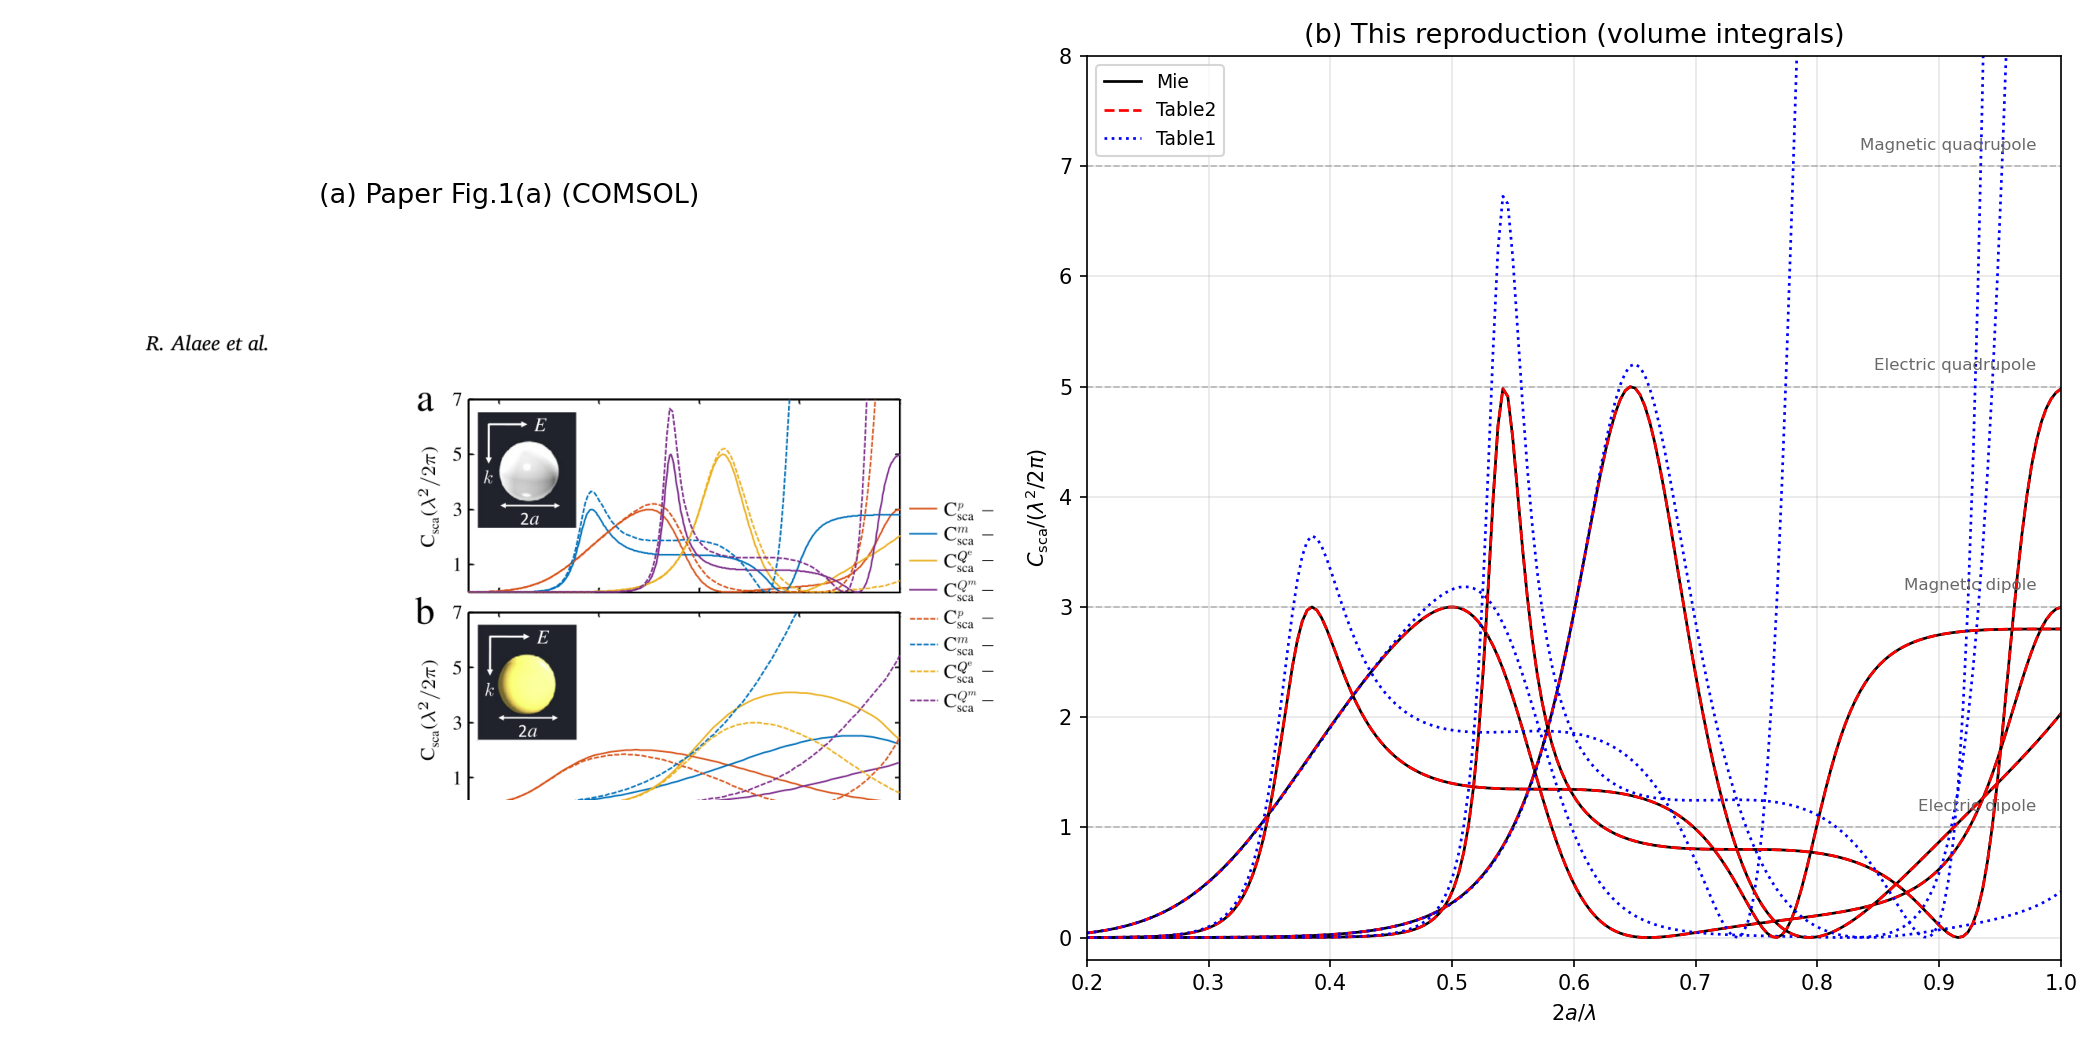
\includegraphics[width=0.82\textwidth]{figs/visual_compare_fig1.png}
\caption{Fig.~1 复现对比：左为复现的散射截面谱（按多极 ED/MD/EQ/MQ 着色），右为 Alaee 2018 Fig.~1 原文（adapted）。两者谱形与峰位一致，误差表是逐通道量化这一致性的结果。}
\label{fig:compare_fig1}
\end{figure}

\textbf{Fig.~2（金球 $a=250$ nm，Johnson--Christy 色散）}：同一方法推广到有损色散材料，加密积分网格（$60\times61\times120$）后：

\begin{center}
\begin{tabular}{cccc}
\toprule
ED & MD & EQ & MQ \\
\midrule
$0.0119\%$ & $0.0170\%$ & $0.0161\%$ & $0.0241\%$ \\
\bottomrule
\end{tabular}
\end{center}

\begin{figure}[H]
\centering
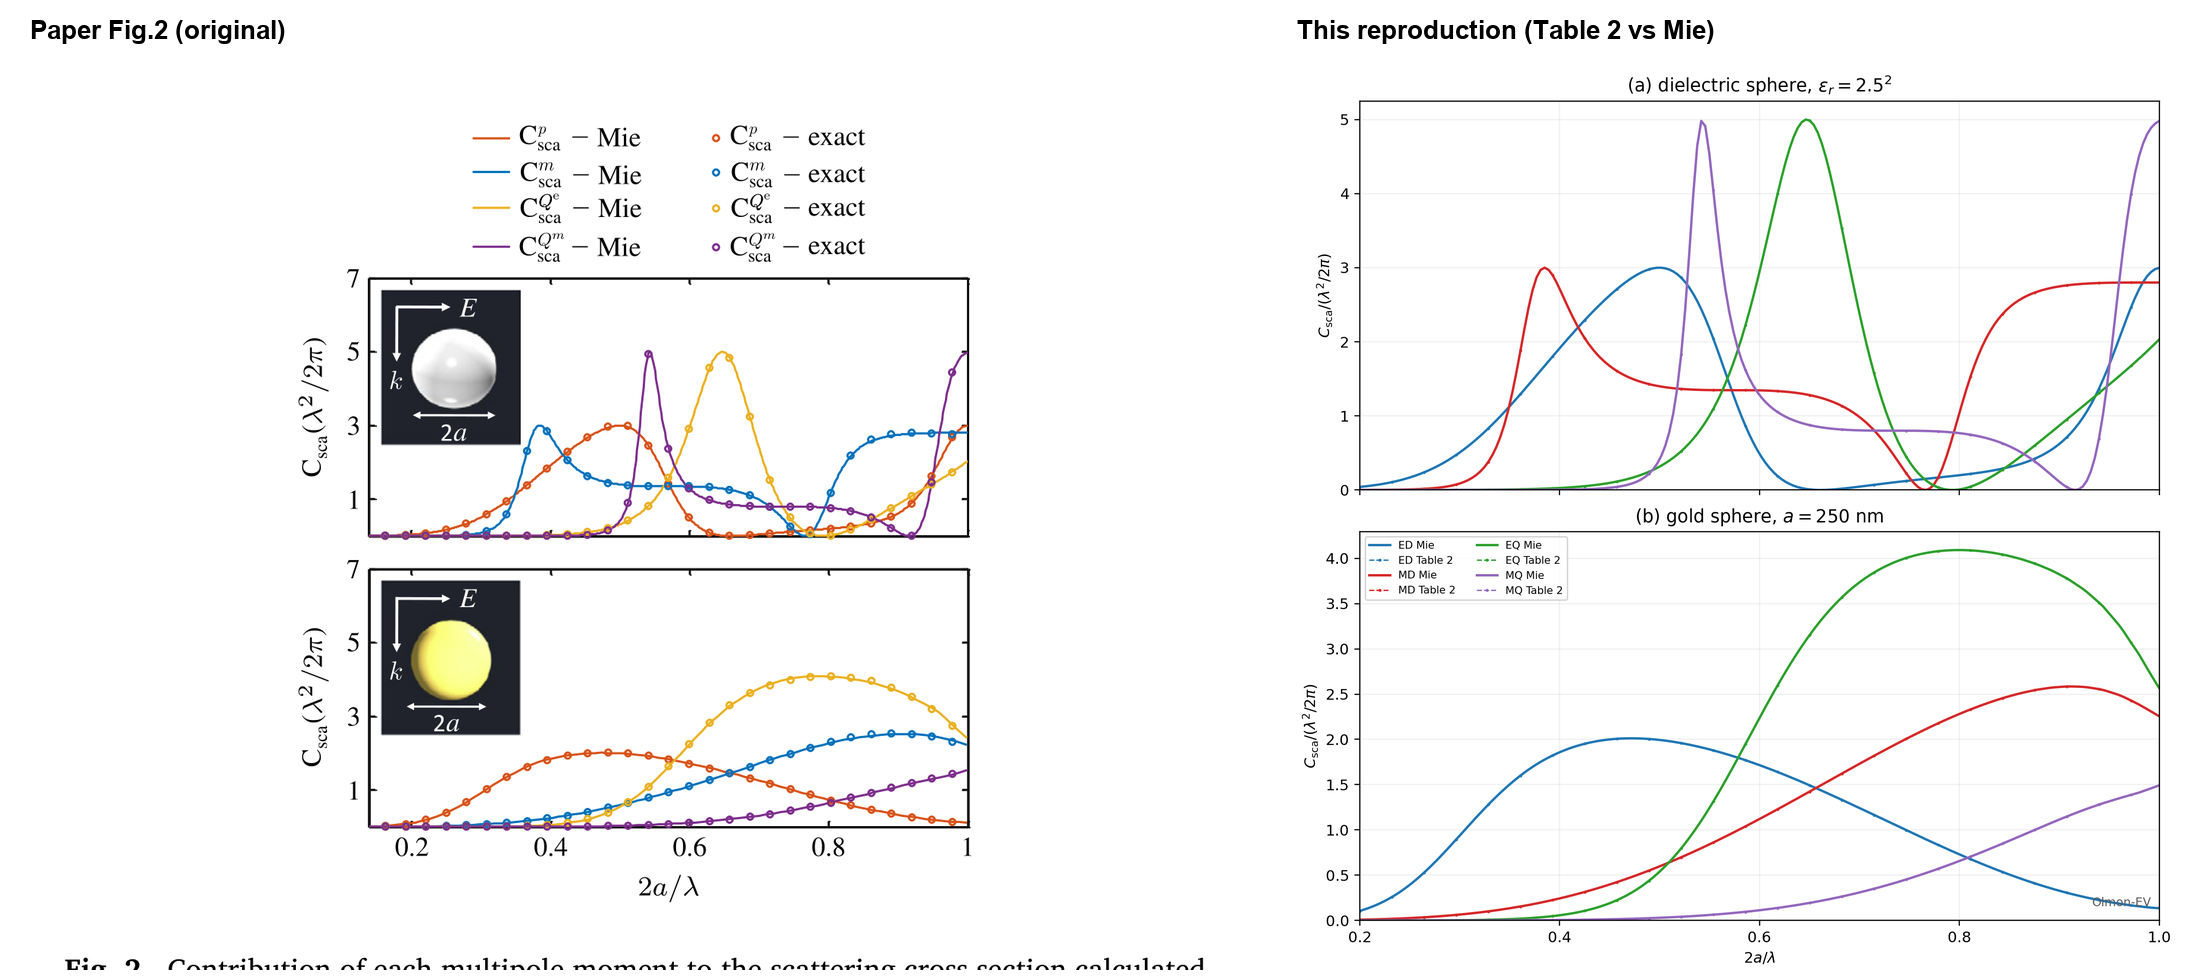
\includegraphics[width=0.82\textwidth]{figs/visual_compare_fig2.png}
\caption{Fig.~2 复现对比：金球多极分解的复现谱（左）与 Alaee 2018 Fig.~2 原文（右，adapted），形态一致，误差 $<0.03\%$。}
\label{fig:compare_fig2}
\end{figure}

验证了 Table 2 精确多极矩在复折射率、宽谱、有损条件下与解析 Mie 解一致。

\subsection{Grahn 2012：电流多极矩到散射系数的映射}

双路径映射 + 逐项数值验证：

\begin{itemize}
  \item \textbf{Path A（长波）} 对 Table 1：总截面最大相对误差 $5.71\times10^{-7}$；
  \item \textbf{Path B（有限核）} 对 Mie：$2.94\times10^{-4}$；
  \item \textbf{逐 $m$ 复系数}：1298 行，最大 $1.52\times10^{-3}$；
  \item \textbf{六个解析电流 fixture}：最大闭式误差 $1.19\times10^{-14}$。
\end{itemize}

验证了从局域电流分布到散射场多极系数的映射（Eq.~(1)--(16)）数值正确。

\subsection{Alaee 2018 Fig.~3：耦合金纳米盘的频域真解}

双金盘（$a=250$ nm、$t=80$ nm、$g=120$ nm）无解析解，用 COMSOL 频域有限元求解。9 点谱（$x=0.26$--$0.42$）显示 ED 主导、MD/EQ 在 $x=0.36$ 磁共振（MD $1.60\times10^{-12}$ m$^2$ 主导、EQ 伴生、MQ $\approx0$），与论文共振形态一致。

\begin{figure}[H]
\centering
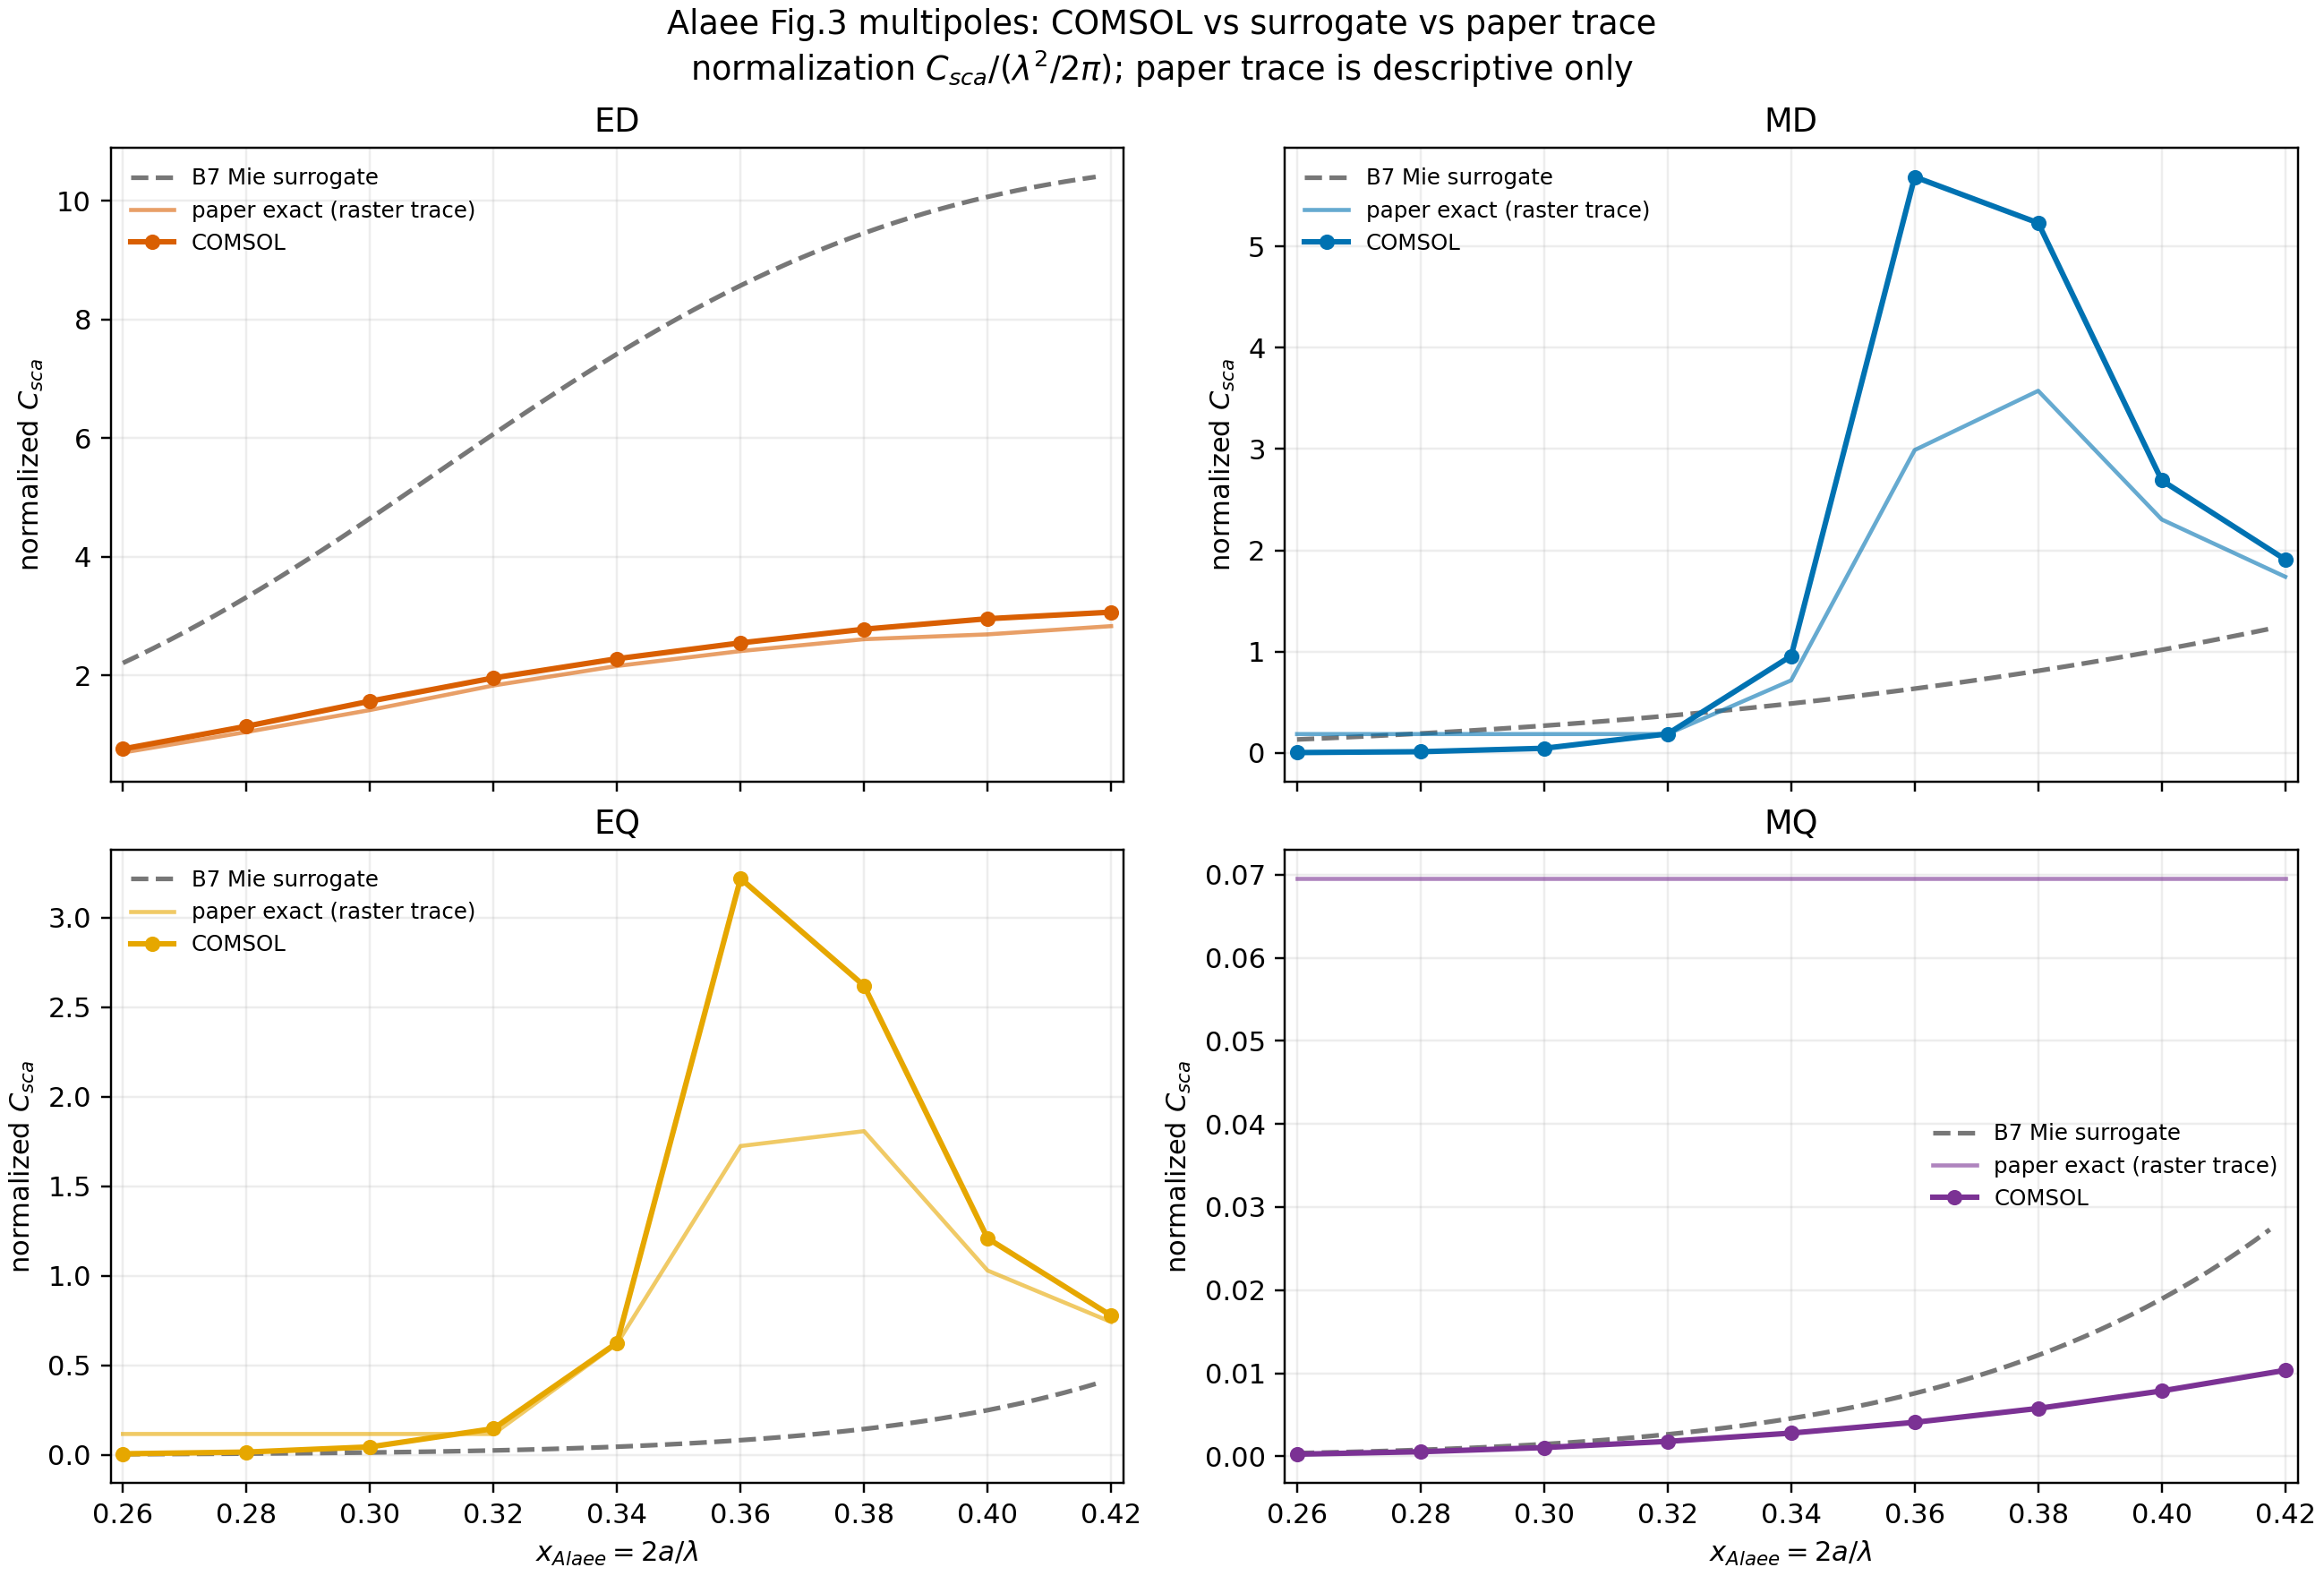
\includegraphics[width=0.82\textwidth]{figs/fig3_comsol_vs_surrogate_paper.png}
\caption{Fig.~3 复现对比：COMSOL 频域 FEM 真解谱（实点）与论文共振形态对照。ED 主导 + MD/EQ 在 $x=0.36$ 磁共振的定性形态一致，峰位偏移 $\sim0.02$--$0.04$、采样 9 点较粗糙（见 §4 与附录 D 的限制说明）。}
\label{fig:compare_fig3}
\end{figure}

$x=0.36$ 四档网格收敛（$1.0\to0.7\to0.5\to0.3$，292,687 至 10,735,163 单元）给出 ED/MQ 已收敛（步进 $<0.26\%$），MD/EQ 步进 $2.26\%/1.95\%$，Richardson 外推收敛阶 $p\approx1.3$（表面场奇异性主导，见 §4.2）。

另以边界元法（RF 模块）同一几何求解，128G 内存跑通（对比有限元 0.3 网格 900G，省约 7 倍），验证边界元作为更省内存的替代路径（PEC 近似下的对比见 §4.1）。
